\tightsection{Quality Improvement via Prediction}
\label{improvement}
Now we can fill in the details of section 3 a bit more.  Figure~\ref{fig:go-overview} shows how prediction and decision-making work in GO.



\begin{figure}[h!]
\centering
 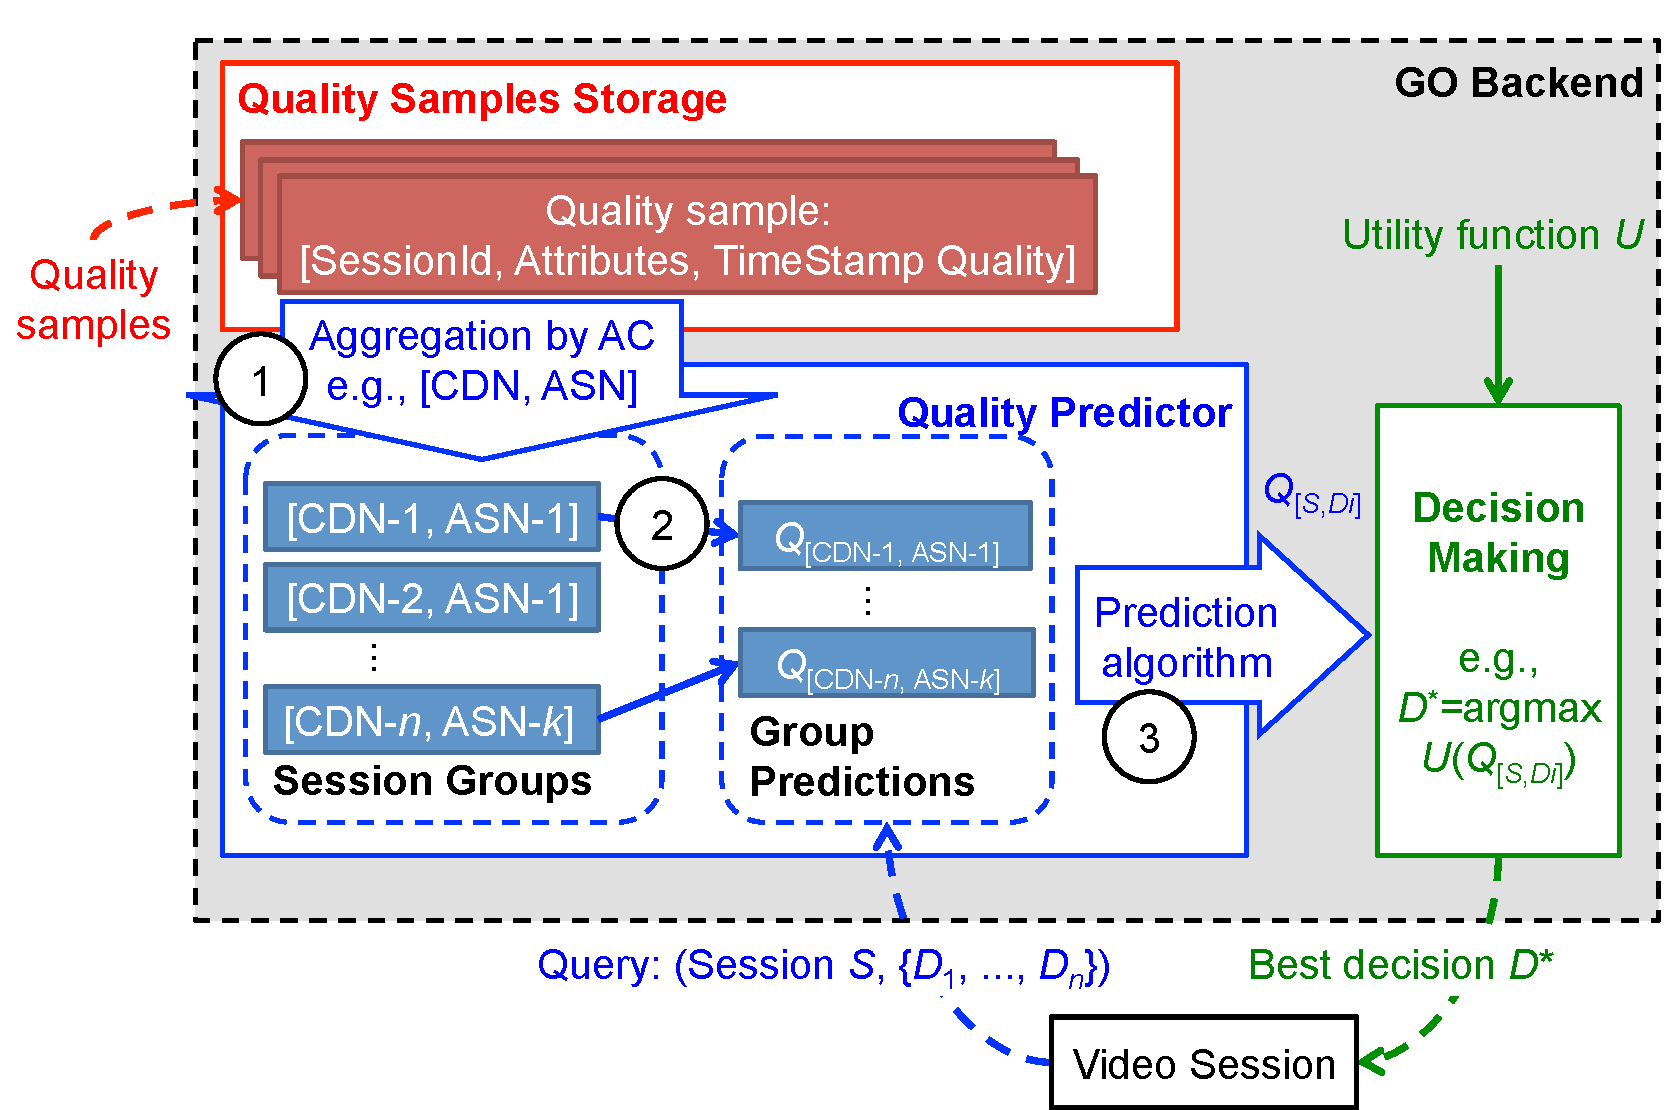
\includegraphics[width=0.5\textwidth] {figures/backend.pdf}
\tightcaption{Schematic overview of GO backend.}
\label{fig:backend}
\end{figure}

\tightsubsection{Behavioral study}
To build confidence in this algorithm, we show how decision-making based on prediction behaves in some simple synthetic scenarios where the optimal decisions are clear:
\begin{packedenumerate}
  \item A sudden change in CDN performance causes relative performance to change.
  \item One CDN performs better for one group (under an observed attribute) and worse for another group.
\end{packedenumerate}
\fillme

\tightsubsection{Evaluation against a baseline}
We show how GO works in practice in a real trace, in comparison to a naive baseline which makes random decisions.  Here we use a methodology similar to A/B testing, which we call {\it counterfactual testing}; the methodology is described in detail in section \ref{sec:counterfactualtesting}.  The dataset is described in section \ref{subsec:dataset}.  Results are displayed in figure \fillme; we can see that \fillme.

\tightsubsection{Synthetic dataset methodology}
Randomized experimentation in real traces is the most important way to evaluate a decision-making algorithm.  However, real traces have a few limitations.  In real traces, it is impractical to identify an optimal alternative against which to compare GO, so that we can understand how close it is to the best algorithm.  In addition, real traces may not contain some rare scenarios of high interest, such as an outage, a rapid change in quality, or a high degree of heterogeneity of quality across spatial groups.  Even when such scenarios are present, they cannot be easily modified to analyze the sensitivity of a decision-making algorithm to the rapidity of changes or the degree of heterogeneity.  To remedy these limitations, we generate a synthetic dataset for a scenario that models some of the important complexities of the real-world dataset.  We analyze the performance of GO in comparison to the oracle.

\fillme

%The scenario is generated as follows: The scenario lasts for $T$ minutes.  Each session is assigned values on four different attributes, $A_0, A_1, B_0,$ and $B_1$, and lasts for $1$ minute.  Each unique attribute combination (i.e. each group) $a$ is associated with some static parameters and some parameters that change over time, which inform the generation of sessions in that group:
%\begin{packedenumerate}
%  \item $n_{a}$: The number of sessions in this group.
%  \item $\mu_{atj}$: The average quality outcome for sessions in this group, when decision $j$ is taken.
%  \item $\sigma_{atj}$: The standard deviation of quality outcomes for sessions in this group, when decision $j$ is taken.
%\end{packedenumerate}

%For each minute $t$, sessions are generated as follows: Group $a$ has $n_{a}$ sessions.  The $i$th session in group $a$ has attribute values $a$.  There are $J$ possible decisions; each session has quality outcome $q_{itaj}$ drawn from the distribution $\operatorname{Normal}(\mu_{atj}, \sigma_{atj}^2)$, for each decision $j$.  The actual decision $d_{ita}$ for the session, which is used to populate the quality sample used in GO, is chosen uniformly at random from among the $J$ possible decisions.

\tightsubsection{Evaluation against an oracle using synthetic data}
Here we compare GO against the oracle in our synthetic scenario.  Show average quality of oracle and GO in the scenario for a reasonably realistic value of the parameters $\lambda$ and $\sigma$, and also for changing values of the parameters (not the full 2D grid, just change one or the other). \fillme

\tightsubsection{Understanding the impact of prediction accuracy on quality improvement}

Separately from the GO algorithm, it is also interesting to see how prediction error impacts quality outcomes in our synthetic scenario.  We add random independent Gaussian noise to the oracle’s predictions (an admittedly crude model of prediction error) and show how larger amounts of noise impact quality outcomes.  Figure \fillme displays this.  We can see that quality improvement is unaffected by small amounts of prediction inaccuracy but drops off quickly at a (scenario-dependent) threshold \fillme.  GO’s performance in quality improvement is equivalent to that of an oracle with \fillme random noise.

While we cannot subtract noise from GO's predictions, we can add Gaussian noise to understand (roughly) the impact of worse prediction.  Figure \fillme displays this for our synthetic scenario, and figure \fillme displays it for a real trace.